\documentclass[12pt, twoside]{article}
\usepackage[letterpaper, margin=1in, head=30pt, headsep=0.1in]{geometry}
\usepackage[english]{babel}
\usepackage[utf8]{inputenc}
\usepackage{amsmath}
\usepackage{amsfonts}
\usepackage{amssymb}
\usepackage{tikz}
\usetikzlibrary{quotes, angles}

\usepackage{graphicx}
\usepackage{enumitem}
\usepackage{multicol}

%\usepackage{pgfplots}
%\pgfplotsset{width=10cm,compat=1.9}
%\usepgfplotslibrary{statistics}
%\usepackage{pgfplotstable}
%\usepackage{tkz-fct}
%\usepackage{venndiagram}

\usepackage{fancyhdr}
\pagestyle{fancy}
\fancyhf{}
\renewcommand{\headrulewidth}{0pt} % disable the underline of the header
\raggedbottom
\newif\ifmeta
\metatrue %print standards and topics tags

\title{Math AI Worksheet Generator and Formative Assessment System}
\author{Chris Huson}
\date{November 2020}

%\fancyhead[RE]{\thepage}
%\fancyhead[RO]{\thepage \\ Name: \hspace{3cm}}
%\fancyhead[L]{BECA / Dr. Huson / 10th Grade Geometry\\* 7 June 2019}
%
%\begin{document}
%\subsubsection*{13.7 Homework: Cross sections, distance applications}
%\fancyhead[L]{BECA / Dr. Huson / Geometry 03-Volume+angle-bisectors\\* pset ID: 34}

\begin{document}

\subsubsection*{4.5 Translation and dilation}
\begin{enumerate}

\item Do Now: A translation maps $A$ to $A'$, as shown, $A(3,1) \rightarrow A'(7,2)$.
\begin{multicols}{2}
  \begin{enumerate}
    \item What is the horizontal shift, how many squares right or left? \vspace{1.25cm}
    \item What is the vertical shift, how many squares up or down? \vspace{1.25cm}
    \item Apply the same translation to $C(1,4)\rightarrow C'(x,y)$. Label the point $C'$ as an ordered pair.
    \end{enumerate}
    \begin{flushright}
    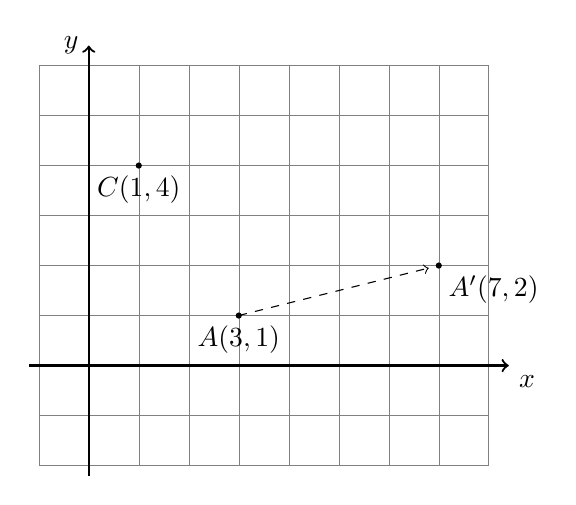
\begin{tikzpicture}[scale=.635]
      \draw [help lines] (-1,-2) grid (8,6);
      \draw [thick, ->] (-1.2,0) -- (8.4,0) node [below right] {$x$};
      \draw [thick, ->] (0,-2.2)--(0,6.4) node [left] {$y$};
      \draw [fill] (3,1) circle [radius=0.05] node[below] {$A(3,1)$};
      \draw [fill] (7,2) circle [radius=0.05] node[below right] {$A'(7,2)$};
      \draw [->, dashed] (3,1)--(6.8,1.95);
      \draw [fill] (1,4) circle [radius=0.05] node[below] {$C(1,4)$};
    \end{tikzpicture}
    \end{flushright}
\end{multicols}

\newpage
\item Vocabulary: A \emph{preimage} is \emph{mapped} to its \emph{image}. For example, triangle $ABC$ undergoes a transformation to make triangle $A'B'C'$.\\[0.5cm]
Translate $\triangle ABC$ by $(x,y) \rightarrow (x+6, y-2)$. Make a table of the coordinates and plot and label the image on the axes.
\begin{flushright}
    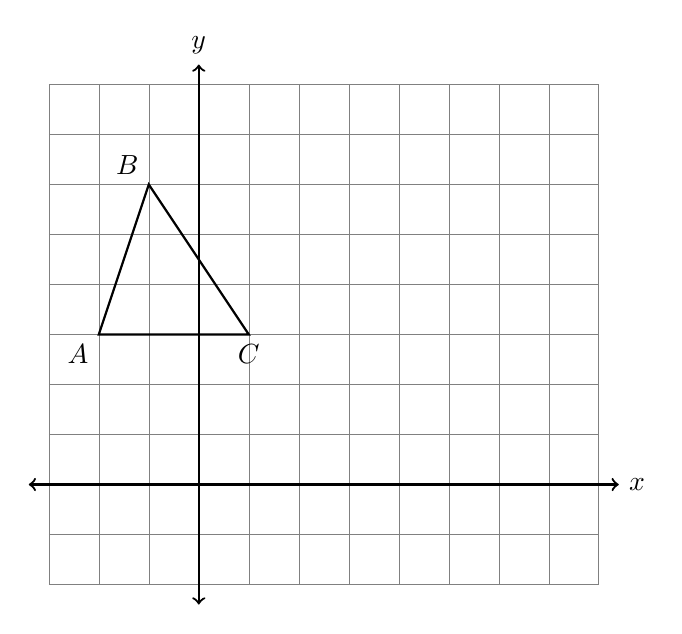
\begin{tikzpicture}[scale=.635]
    \draw [help lines] (-3,-2) grid (8,8);
    \draw [thick, <->] (-3.4,0) -- (8.4,0) node [right] {$x$};
    \draw [thick, <->] (0,-2.4)--(0,8.4) node [above] {$y$};  
    \draw [thick]
      (-2,3) node[below left] {$A$}--
      (-1,6) node[above left] {$B$}--
      (1,3) node[below] {$C$}--cycle;  
  \end{tikzpicture}
\end{flushright}

\newpage
\item Vocabulary: A translation is a \emph{rigid motion}, lengths and angles stay the same. \emph{Corresponding} parts are congruent. \\[0.5cm]
A translation maps triangle $KLM$ onto triangle $PQR$. \vspace{0.5cm}
    \begin{multicols}{2}
      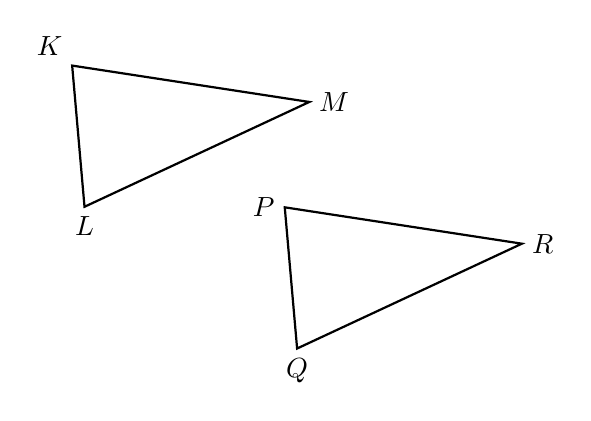
\begin{tikzpicture}[scale=0.9]
        \coordinate [label=above left:$K$](A) at (95:2);
        \coordinate [label=below:$L$](B) at (0, 0);
        \coordinate [label=right:$M$](C) at (25:3.5);
        \draw [thick] (A)--(B)--(C)--cycle;
        \draw [thick, xshift=3cm, yshift=-2cm] (95:2) node[left]{$P$}--
        (0,0) node[below]{$Q$}--
        (25:3.5) node[right]{$R$}--cycle;
      \end{tikzpicture}\\
      Write each corresponding object.
      \begin{enumerate}
        \item $L \rightarrow$ \rule{2cm}{0.15mm}
        \item $\angle M \cong$ \rule{2cm}{0.15mm}
        \item $\overline {LM} \cong$ \rule{2cm}{0.15mm}
        \item Justify $\triangle KLM \cong \triangle PQR$. Use the words ``rigid motion" and ``translation''.
      \end{enumerate}
    \end{multicols}

\newpage
\item Vocabulary: A dilation stretches or shrinks. It has a \emph{center} and a \emph{scale factor, k}. \\[0.5cm]
A dilation centered at $A$ with scale factor $k=2$ maps $\triangle ABC \rightarrow \triangle ADE$. Given the sides of the preimage, $AC = 4$, $BC = 3$, $AB = 5$. \\[0.5cm]
$DE = 6$, how long are $AD$ and $AE$?
    \begin{flushright}
      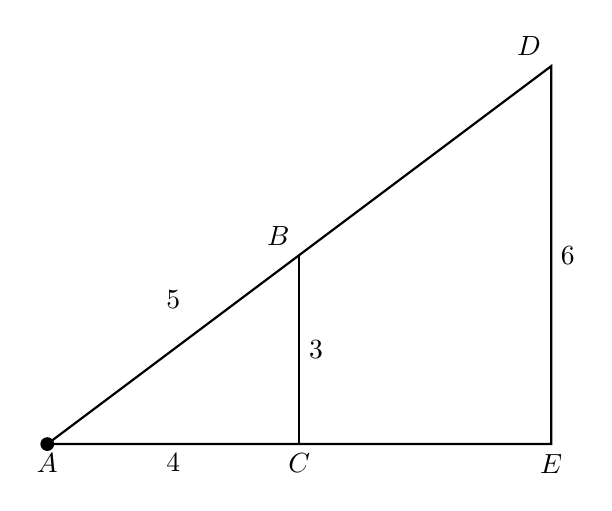
\begin{tikzpicture}[scale=0.8]
        \draw [-, thick] (0,0)--
        (8,0) node[below]{$E$}--
        (8,6) node[above left]{$D$}--cycle;
        \draw [thick] (4,0)--(4,3);
        \draw [fill] (0,0) circle [radius=0.1] node[below] {$A$};
        \node at (4,0) [below]{$C$};
        \node at (4,3) [above left]{$B$};
        \node at (2, 0) [below]{$4$};
        \node at (2, 2) [above]{$5$};
        \node at (8, 3) [right]{$6$};
        \node at (4, 1.5) [right]{$3$};
      \end{tikzpicture}
    \end{flushright}

\newpage
\item Perform a dilation in Geogebra and insert the image on this slide. Be sure to label the points, and fully describe the dilation. (specify its center and scale factor $k$)


\end{enumerate}
\end{document}